\documentclass[12pt]{report}
\usepackage[utf8]{inputenc}
\usepackage[russian]{babel}
%\usepackage[14pt]{extsizes}
\usepackage{listings}
\usepackage{graphicx}
\usepackage{amsmath,amsfonts,amssymb,amsthm,mathtools} 
\usepackage{pgfplots}
\usepackage{filecontents}
\usepackage{float}
\usepackage{indentfirst}
\usepackage{eucal}
\usepackage{enumitem}
\frenchspacing

\usepackage{indentfirst} % Красная строка


\usetikzlibrary{datavisualization}
\usetikzlibrary{datavisualization.formats.functions}

\usepackage{amsmath}




% Для листинга кода:
\lstset{ %
language=haskell,                 % выбор языка для подсветки (здесь это С)
basicstyle=\small\sffamily, % размер и начертание шрифта для подсветки кода
numbers=left,               % где поставить нумерацию строк (слева\справа)
numberstyle=\tiny,           % размер шрифта для номеров строк
stepnumber=1,                   % размер шага между двумя номерами строк
numbersep=5pt,                % как далеко отстоят номера строк от подсвечиваемого кода
showspaces=false,            % показывать или нет пробелы специальными отступами
showstringspaces=false,      % показывать или нет пробелы в строках
showtabs=false,             % показывать или нет табуляцию в строках
frame=single,              % рисовать рамку вокруг кода
tabsize=2,                 % размер табуляции по умолчанию равен 2 пробелам
captionpos=t,              % позиция заголовка вверху [t] или внизу [b] 
breaklines=true,           % автоматически переносить строки (да\нет)
breakatwhitespace=false, % переносить строки только если есть пробел
escapeinside={\#*}{*)}   % если нужно добавить комментарии в коде
}

\usepackage[left=2cm,right=2cm, top=2cm,bottom=2cm,bindingoffset=0cm]{geometry}
% Для измененных титулов глав:
\usepackage{titlesec, blindtext, color} % подключаем нужные пакеты
\definecolor{gray75}{gray}{0.75} % определяем цвет
\newcommand{\hsp}{\hspace{20pt}} % длина линии в 20pt
% titleformat определяет стиль
\titleformat{\chapter}[hang]{\Huge\bfseries}{\thechapter\hsp\textcolor{gray75}{|}\hsp}{0pt}{\Huge\bfseries}


% plot
\usepackage{pgfplots}
\usepackage{filecontents}
\usetikzlibrary{datavisualization}
\usetikzlibrary{datavisualization.formats.functions}

\begin{document}
%\def\chaptername{} % убирает "Глава"
\thispagestyle{empty}
\begin{titlepage}
	\noindent \begin{minipage}{0.15\textwidth}
	
\includegraphics[width=\linewidth]{img/b_logo}
	\end{minipage}
	\noindent\begin{minipage}{0.9\textwidth}\centering
		\textbf{Министерство науки и высшего образования Российской Федерации}\\
		\textbf{Федеральное государственное бюджетное образовательное учреждение высшего образования}\\
		\textbf{~~~«Московский государственный технический университет имени Н.Э.~Баумана}\\
		\textbf{(национальный исследовательский университет)»}\\
		\textbf{(МГТУ им. Н.Э.~Баумана)}
	\end{minipage}
	
	\noindent\rule{18cm}{3pt}
	\newline\newline
	\noindent ФАКУЛЬТЕТ $\underline{\text{«Информатика и системы управления»}}$ \newline\newline
	\noindent КАФЕДРА $\underline{\text{«Программное обеспечение ЭВМ и информационные технологии»}}$\newline\newline\newline\newline\newline
	
	
	\begin{center}
		\noindent\begin{minipage}{1.3\textwidth}\centering
			\Large\textbf{  Отчет по лабораторной работе №4}\newline
			\textbf{по дисциплине "Операционные системы"}\newline\newline
		\end{minipage}
	\end{center}
	
	\noindent\textbf{Тема} $\underline{\text{Процессы. Системные вызовы fork() и exec()}}$\newline\newline
	\noindent\textbf{Студент} $\underline{\text{Романов А.В.~~~~~~~~~~~~~~~~~~~~~~~~~~~~~~~~~~~~~~}}$\newline\newline
	\noindent\textbf{Группа} $\underline{\text{ИУ7-53Б~~~~~~~~~~~~~~~~~~~~~~~~~~~~~~~~~~~~~~~~~~~~~~}}$\newline\newline
	\noindent\textbf{Оценка (баллы)} $\underline{\text{~~~~~~~~~~~~~~~~~~~~~~~~~~~~~~~~~~~~~~~~~~~~~}}$\newline\newline
	\noindent\textbf{Преподаватели} $\underline{\text{Рязанова Н.Ю.~~~~~~~~~~~~~~~~~~~~~~~~~~}}$\newline\newline\newline
	
	\begin{center}
		\vfill
		Москва~---~\the\year
		~г.
	\end{center}
\end{titlepage}

\newpage

\section*{Задание №1}

Процессы-сироты. В программе создаются не менее двух потомков. В потомках вызывается sleep(), чтобы предок гарантированно завершился
раньше своих потомков. Продемонстрировать с помощью соответствующего вывода информацию об идентификаторах процессов и их группе.

\begin{lstlisting}[label=some-code,caption=Процессы-сироты,language=C]
#include <stdio.h>
#include <unistd.h>

#define OK 0
#define FORK_FAILURE 1

#define N 2
#define SLP_INTV 2

int main()
{
	int child[N];
	int pid;
	fprintf(stdout, "Parent process. PID: %d, GROUP: %d\n", getpid(), getpgrp());

	for (size_t i = 0; i < N; i++)
	{
		pid = fork();
		if (-1 == pid)
		{
			perror("Cant fork.");
			return FORK_FAILURE;
		}
		else if (0 == pid)
		{
			sleep(SLP_INTV);
			fprintf(stdout, "Child process #%d. PID: %d, PPID: %d, GROUP: %d\n", i + 1, getpid(), getppid(), getpgrp());
			return OK;
		} else

		{
			child[i] = pid;
		}
	}
	
	fprintf(stdout, "Parent process. Children ID: %d, %d.\nParent process is dead.\n", child[0], child[1]);
	return OK;
}
\end{lstlisting}

\begin{figure}[H]

	\centering

	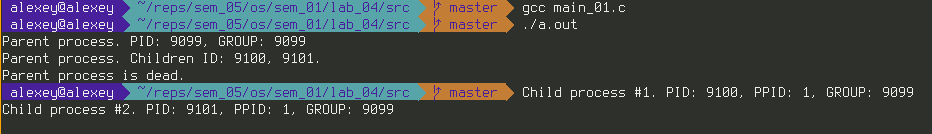
\includegraphics[width=\linewidth]{img/task01.png}
	\caption{Демонстрация работы программы (задание №1).}

	\label{fig:task01}

\end{figure}

\section*{Задание №2}

Предок ждет завершения своих потомком, используя системный вызов
wait(). Вывод соответствующих сообщений на экран.

\begin{lstlisting}[label=some-code,caption=Вызов функции wait(),language=C]
#include <stdio.h>
#include <unistd.h>
#include <sys/types.h>
#include <sys/wait.h>

#define OK 0
#define FORK_FAILURE 1

#define N 2
#define SLP_INTV 2

int main()

{
	int child[N];
	int pid;
	
	fprintf(stdout, "Parent process. PID: %d, GROUP: %d\n", getpid(), getpgrp());
	
	for (size_t i = 0; i < N; i++)
	{
		pid = fork();
		
		if (-1 == pid)
		{
			perror("Cant fork.");
			return FORK_FAILURE;
		}
		else if (0 == pid)
		{
			sleep(SLP_INTV);
			fprintf(stdout, "Child process #%d. PID: %d, PPID: %d, GROUP: %d\n", i + 1, getpid(), getppid(), getpgrp());
			return OK;
		} else
		{
			child[i] = pid;
		}

	}

	
	for (size_t i = 0; i < N; i++)
	{
		int status, statval;
		
		pid_t childpid = wait(&status);
		fprintf(stdout, "Child process (PID %d) finished. Status: %d\n", childpid, status);
		
		if (WIFEXITED(statval))
		{
			fprintf(stdout, "Child process finished with code: %d\n", WEXITSTATUS(statval));
		}
		else
		{
			fprintf(stdout, "Child process terminated abnormally\n");
		}
		
	}
	
	fprintf(stdout, "Parent process. Children ID: %d, %d.\nParent process is dead.\n", child[0], child[1]);
	
	return OK;
}
\end{lstlisting}

\begin{figure}[H]

	\centering

	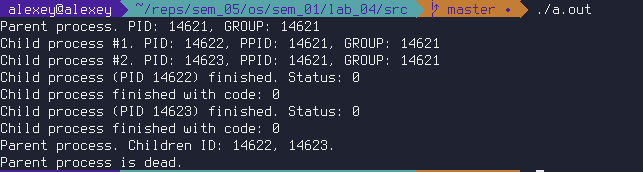
\includegraphics[width=\linewidth]{img/task02.png}
	\caption{Демонстрация работы программы (задание №2).}

	\label{fig:task02}

\end{figure}

\section*{Задание №3}

Потомки переходят на выполнение других программ. Предок ждет завершения своих потомков. Вывод соответствующих сообщений на экран.

\begin{lstlisting}[label=some-code,caption=Вызов функции execlp(),language=C]
#include <stdio.h>
#include <unistd.h>
#include <sys/types.h>
#include <sys/wait.h>

#define OK 0
#define FORK_FAILURE 1

#define N 2
#define SLP_INTV 2

int main()
{
	int child[N];
	int pid;
	
	fprintf(stdout, "Parent process. PID: %d, GROUP: %d\n", getpid(), getpgrp());
	
	for (size_t i = 0; i < N; i++)
	{
		pid = fork();
		
		if (-1 == pid)
		{
			perror("Cant fork.");
			return FORK_FAILURE;
		}
		else if (0 == pid)
		{
			sleep(SLP_INTV);
			fprintf(stdout, "Child process #%d. PID: %d, PPID: %d, GROUP: %d\n", i + 1, getpid(), getppid(), getpgrp());
			
			int rc = execlp(commands[i], commands[i], 0);
			
			if (-1 == rc)
			{
				perror("Cant exec.");
				return EXEC_FAILURE;
			}
			
			
			return OK;
		} else
		{
			child[i] = pid;
		}
	}
	
	for (size_t i = 0; i < N; i++)
	{
		int status, statval;
		
		pid_t childpid = wait(&status);
		fprintf(stdout, "Child process (PID %d) finished. Status: %d\n", childpid, status);
		
		if (WIFEXITED(statval))
		{
			fprintf(stdout, "Child process finished with code: %d\n", WEXITSTATUS(statval));
		}
		else
		{
			fprintf(stdout, "Child process terminated abnormally\n");
		}
	}
	
	fprintf(stdout, "Parent process. Children ID: %d, %d.\nParent process is dead.\n", child[0], child[1]);
	
	return OK;
}
\end{lstlisting}

\begin{figure}[H]

	\centering

	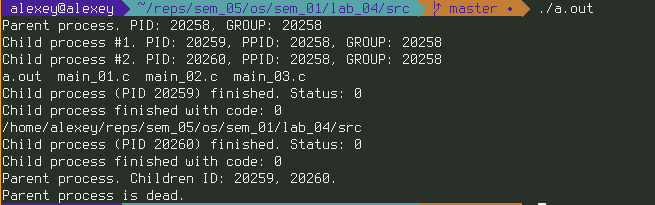
\includegraphics[width=\linewidth]{img/task03.png}
	\caption{Демонстрация работы программы (задание №3).}

	\label{fig:task03}

\end{figure}

\section*{Задание №4}

Предок и потомки обмениваются сообщениями через неименованный
программный канал. Предок ждет завершения своих потомков. Вывод соответствующих сообщений на экран.

\begin{lstlisting}[label=some-code,caption=Использование pipe,language=C]
#include <stdio.h>
#include <unistd.h>
#include <string.h>
#include <sys/types.h>
#include <sys/wait.h>

#define OK 0
#define FORK_FAILURE 1
#define EXEC_FAILURE 2
#define PIPE_FAILURE 3

#define N 2
#define SLP_INTV 2
#define BUFFSIZE 128

int main()
{
	int child[N];
	int fd[N];
	int pid;
	
	const char *const messages[N] = { "First message!\n", \"Second message!\n" };
	char buffer[BUFFSIZE] = { 0 };
	
	if (-1 == pipe(fd))
	{
		perror("Cant pipe.");
		return PIPE_FAILURE;
	}
	
	fprintf(stdout, "Parent process. PID: %d, GROUP: %d\n", getpid(), getpgrp());
	
	for (size_t i = 0; i < N; i++)
	{
		pid = fork();
		
		if (-1 == pid)
		{
			perror("Cant fork.");
			return FORK_FAILURE;
		}
		else if (0 == pid)
		{
			close(fd[0]);
			write(fd[1], messages[i], strlen(messages[i]));
			fprintf(stdout, "Message #%d sent to parent!\n", i + 1);
			
			return OK;
		}
		else
		{
			child[i] = pid;
		}
	}
	
	for (size_t i = 0; i < N; i++)
	{
		int status, statval;
		
		pid_t childpid = wait(&status);
		fprintf(stdout, "Child process (PID %d) finished. Status: %d\n", childpid, status);
		
		if (WIFEXITED(statval))
		{
			fprintf(stdout, "Child process finished with code: %d\n", WEXITSTATUS(statval));
		}
		else
		{
			fprintf(stdout, "Child process terminated abnormally\n");
		}
	}
	
	close(fd[1]);
	read(fd[0], buffer, BUFFSIZE);
	
	fprintf(stdout, "Received messages:\n%s", buffer);
	fprintf(stdout, "Parent process. Children ID: %d, %d.\nParent process is dead.\n", child[0], child[1]);
	
	return OK;
}
\end{lstlisting}

\begin{figure}[H]

	\centering

	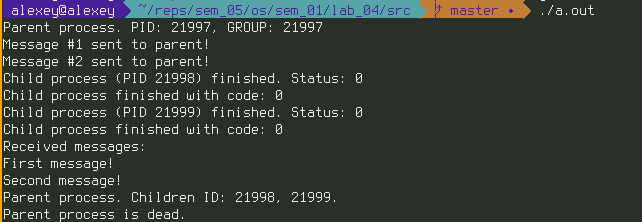
\includegraphics[width=\linewidth]{img/task04.png}
	\caption{Демонстрация работы программы (задание №4).}

	\label{fig:task04}

\end{figure}

\section*{Задание №5}

Предок и потомки обмениваются сообщениями через неименованный
программный канал. С помощью сигнала меняется ход выполнения программы. Предок ждет завершения своих потомков. Вывод соответствующих сообщений на экран.

\begin{lstlisting}[label=some-code,caption=Использование сигналов,language=C]
\end{lstlisting}

\begin{figure}[H]

	\centering

	%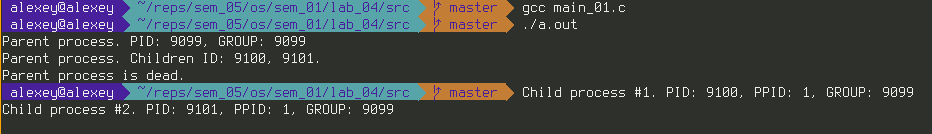
\includegraphics[width=\linewidth]{img/task01.png}
	\caption{Демонстрация работы программы (задание №5).}

	\label{fig:task05_01}

\end{figure}

\begin{figure}[h]

	\centering

	%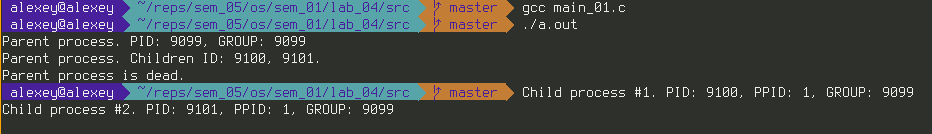
\includegraphics[width=\linewidth]{img/task01.png}
	\caption{Демонстрация работы программы (задание №5).}

	\label{fig:task05_02}

\end{figure}


\bibliographystyle{utf8gost705u}  % стилевой файл для оформления по ГОСТу

\bibliography{51-biblio}          % имя библиографической базы (bib-файла)


\end{document}
